%%%%%%%%%%%%%%%%%%%% main.tex %%%%%%%%%%%%%%%%%%%%%%%%%%%%%%%%%%%%%%
%
% PiyaNota -- WCTP 2026 abstract, typeset with the Springer SVProc class
% (LaTeX2e, based on LaTex_Package/templates/author.tex).
%
% Page 1 = abstract page, page 2 = supporting material. Each must stay
% exactly one page. If page 2 overflows after compiling, lower
% \FigOneWidth and/or \FigTwoHeight below before touching the text.
%
%%%%%%%%%%%%%%%% Springer %%%%%%%%%%%%%%%%%%%%%%%%%%%%%%%%%%%%%%%%%%%

\documentclass{svproc}

% RECOMMENDED (from the template): typeset URLs, URIs, and DOIs
\usepackage{url}
\def\UrlFont{\rmfamily}

\usepackage[T1]{fontenc}
\usepackage{graphicx}
\usepackage{float}      % [H] keeps figures/table on the supporting page
\usepackage{booktabs}
\graphicspath{{figures/}}

% --- Page-2 fit knobs -------------------------------------------------
\newcommand{\FigOneWidth}{0.62\textwidth}   % Figure 1 (pipeline)
\newcommand{\FigTwoHeight}{2.7cm}           % each panel of Figure 2
% ----------------------------------------------------------------------

% Lets \caption inside a plain minipage be numbered as a figure, so
% Figure 2 can sit beside text without being a float.
\makeatletter
\newcommand{\figurecaptype}{\def\@captype{figure}}
\makeatother

\begin{document}
\mainmatter              % start of a contribution
\pagestyle{empty}        % no running heads/page numbers on a 2-page abstract
%
\title{PiyaNota: A Mobile Application for Optical Music Recognition and
Piano Audio Rendering of Filipino SATB Choral Sheet Music}
%
\titlerunning{PiyaNota}
%
\author{Paula Sophia V. Macalindong \and Tita R. Herradura}
%
\authorrunning{P.\,S.\,V. Macalindong and T.\,R. Herradura}
%
\tocauthor{Paula Sophia V. Macalindong and Tita R. Herradura}
%
\institute{College of Information and Computer Studies,\\
De La Salle University -- Dasmari\~nas,\\
Dasmari\~nas, Cavite, Philippines}

\maketitle
\thispagestyle{empty}

\begin{abstract}
Choral singing is prevalent in Filipino culture, practiced in worship
services, schools, and community choirs, yet many choir members have
limited music-reading skills and learn parts from conductors. Existing
tools fall short: Optical Music Recognition (OMR) models degrade on
photos, commercial apps assume musical literacy, SkiMusic, a
Filipino-developed system, applies fixed rules to piano scores only, and
no annotated Filipino SATB dataset exists. We present PiyaNota, an
Android app converting photos of open-score SATB (Soprano, Alto, Tenor,
Bass) scores into per-voice piano audio. YOLOv8 isolates staves, and a
convolutional recurrent network fine-tuned on multi-font renderings, with
a clef and key-signature classifier, transcribes them. In a 12-page pilot
evaluation, all 100 staves were detected; camera pitch accuracy rose from
under 5\% before fine-tuning to 83.3--83.4\% (88.7--89.1\% digital),
though music symbol error rate remains 33.8--34.8\%. PiyaNota offers an
annotated Filipino SATB dataset, a deep learning pipeline, and an app for
untrained singers.
\keywords{Optical Music Recognition, Computer Vision, Deep Learning,
Mobile Application, Filipino Choral Music, Musical Literacy}
\end{abstract}

\section*{Contact Author/s}
% Two authors side by side to keep the abstract page to one page.
\noindent
\begin{minipage}[t]{0.49\textwidth}
\small\raggedright
\textbf{Name:} Paula Sophia V. Macalindong\\
Student Author, BS Computer Science with Specialization in
Intelligent Systems, 4th Year\\
\textbf{Phone:} 09190747420\\
\textbf{Email:} \email{MPV0154@dlsud.edu.ph}
\end{minipage}\hfill
\begin{minipage}[t]{0.47\textwidth}
\small\raggedright
\textbf{Name:} Tita R. Herradura\\
Adviser, College of Information and Computer Studies\\
\textbf{Phone:} 09234019514\\
\textbf{Email:} \email{TRHerradura@dlsud.edu.ph}
\end{minipage}

%%%%%%%%%%%%%%%%%%%%%%%%%%% PAGE 2 %%%%%%%%%%%%%%%%%%%%%%%%%%%%%%%%%%%
\newpage
\thispagestyle{empty}
% svproc puts 8mm above and below every in-text float; on a one-page
% supporting sheet that alone costs ~3cm, so tighten it here only.
\setlength{\intextsep}{2mm plus 1pt minus 1pt}
\setlength{\abovecaptionskip}{4pt}

\section*{Supporting Material: PiyaNota Work-in-Progress Status}

\subsection*{1.\enspace System Overview and Development Status}

\begin{figure}[H]
\centering
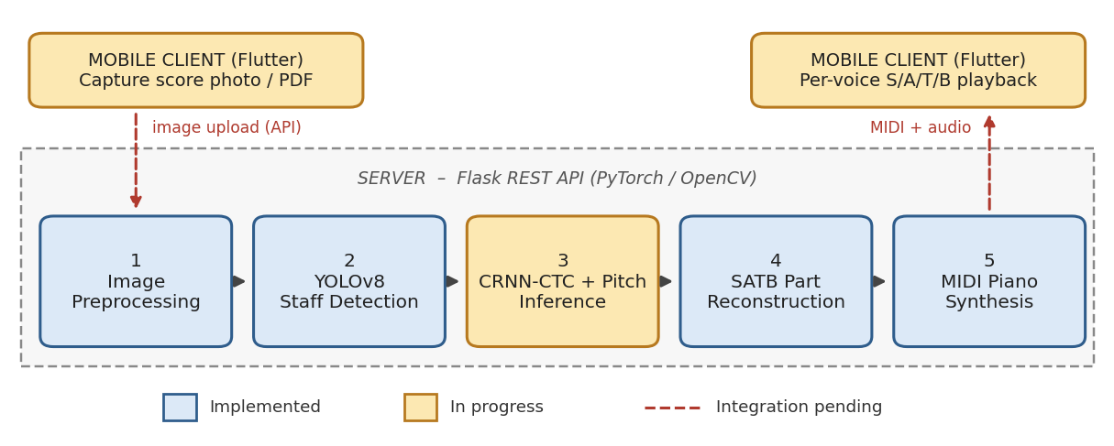
\includegraphics[width=\FigOneWidth]{fig1_pipeline.png}
\caption{PiyaNota pipeline: mobile capture, five-stage server-side
processing, and per-voice audio playback.}
\label{fig:pipeline}
\end{figure}

\subsection*{2.\enspace Preliminary Results: Camera-Captured vs.\
Digital Input}

\begin{table}[H]
\caption{Final system (fine-tuned CRNN-CTC + clef/key classifier) on 12
test pages (100 staves, 1,008 notes per condition). Ranges span two
training seeds. Staff detection = share of staves found and assigned the
correct voice; pitch accuracy ignores note duration; lower SER is
better.}
\label{tab:results}
\centering
\small
\begin{tabular}{@{}lccc@{}}
\toprule
Input Condition & Staff Detection & Symbol Error & Pitch Inference \\
                & (recall)        & Rate (SER)   & Acc.            \\
\midrule
Digital (PDF render)  & 100.0\% & 25.0--25.5\% & 88.7--89.1\% \\
Camera-captured photo & 100.0\% & 33.8--34.8\% & 83.3--83.4\% \\
\midrule
Degradation ($\Delta$) & 0.0\,pp & $+8.8$ to $+9.2$\,pp
                       & $-5.4$ to $-5.7$\,pp \\
\bottomrule
\end{tabular}
\end{table}

% Figure 2 sits beside the discussion paragraph (instead of full width)
% so the supporting material fits on a single page.
\noindent
\begin{minipage}[t]{0.62\textwidth}
\vspace{0pt}
The initial pipeline (CRNN-CTC trained only on single-font synthetic
data) detected 84.0\% of staves on digital and 56.0\% on camera input,
with pitch accuracy below 5\% in both because it read no clef
correctly. Pitch accuracy does not penalise extra notes: about one in
three predicted notes is spurious or wrong-pitched (note precision
66--69\%).
\end{minipage}\hfill
\begin{minipage}[t]{0.36\textwidth}
\vspace{0pt}
\centering
\begin{tabular}{@{}c@{\hspace{4pt}}c@{}}
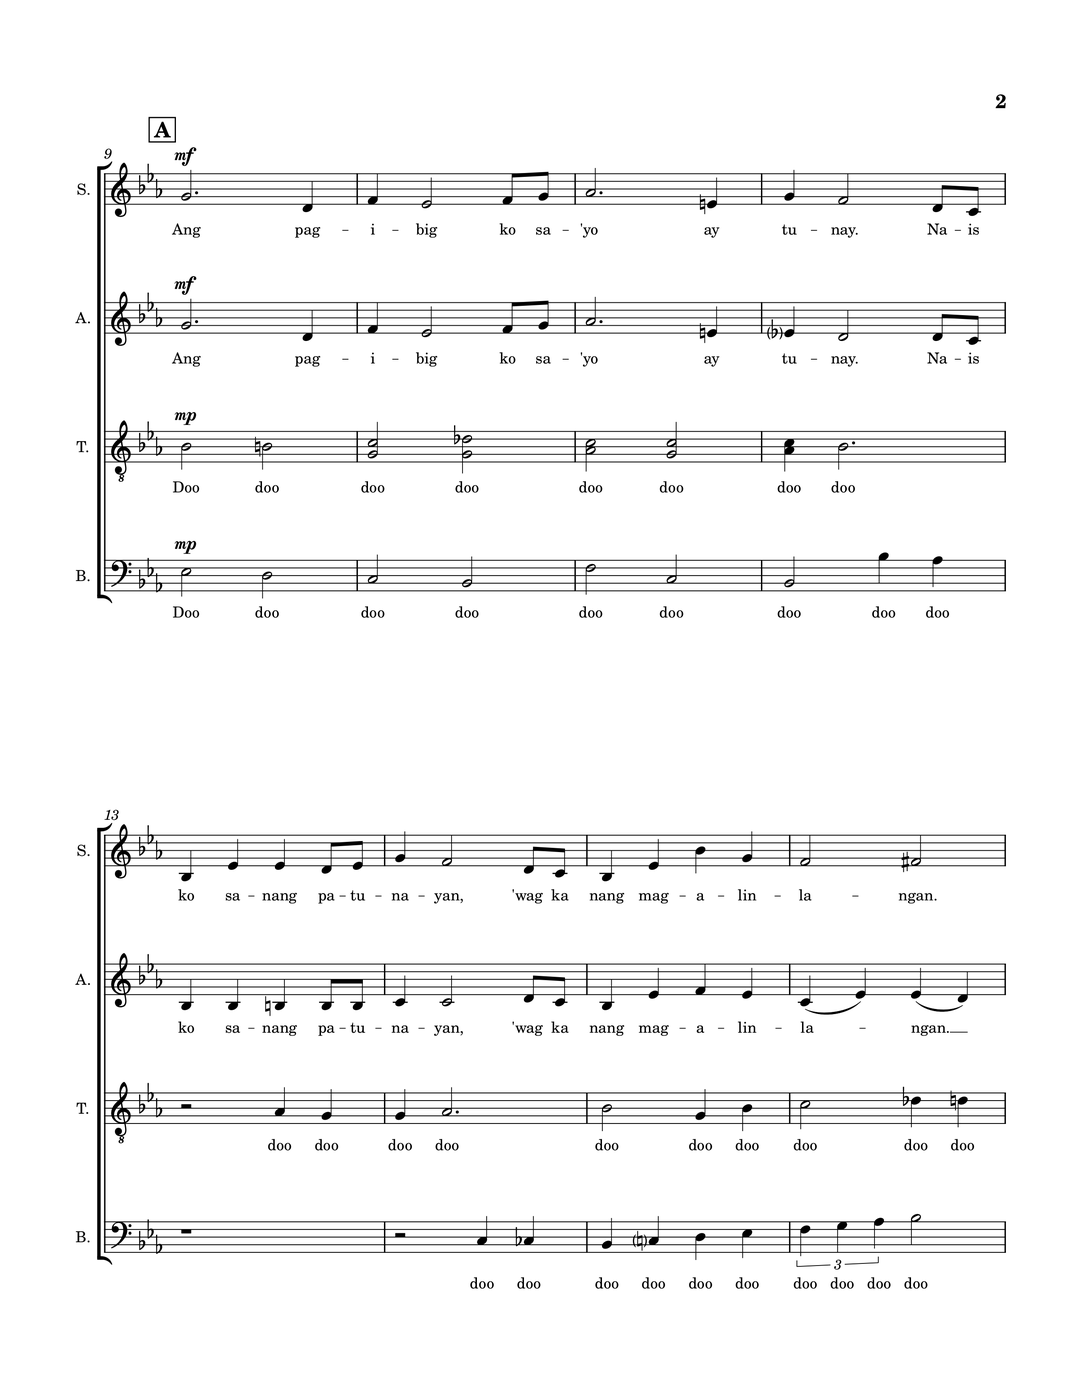
\includegraphics[height=\FigTwoHeight]{fig2a_digital.png} &
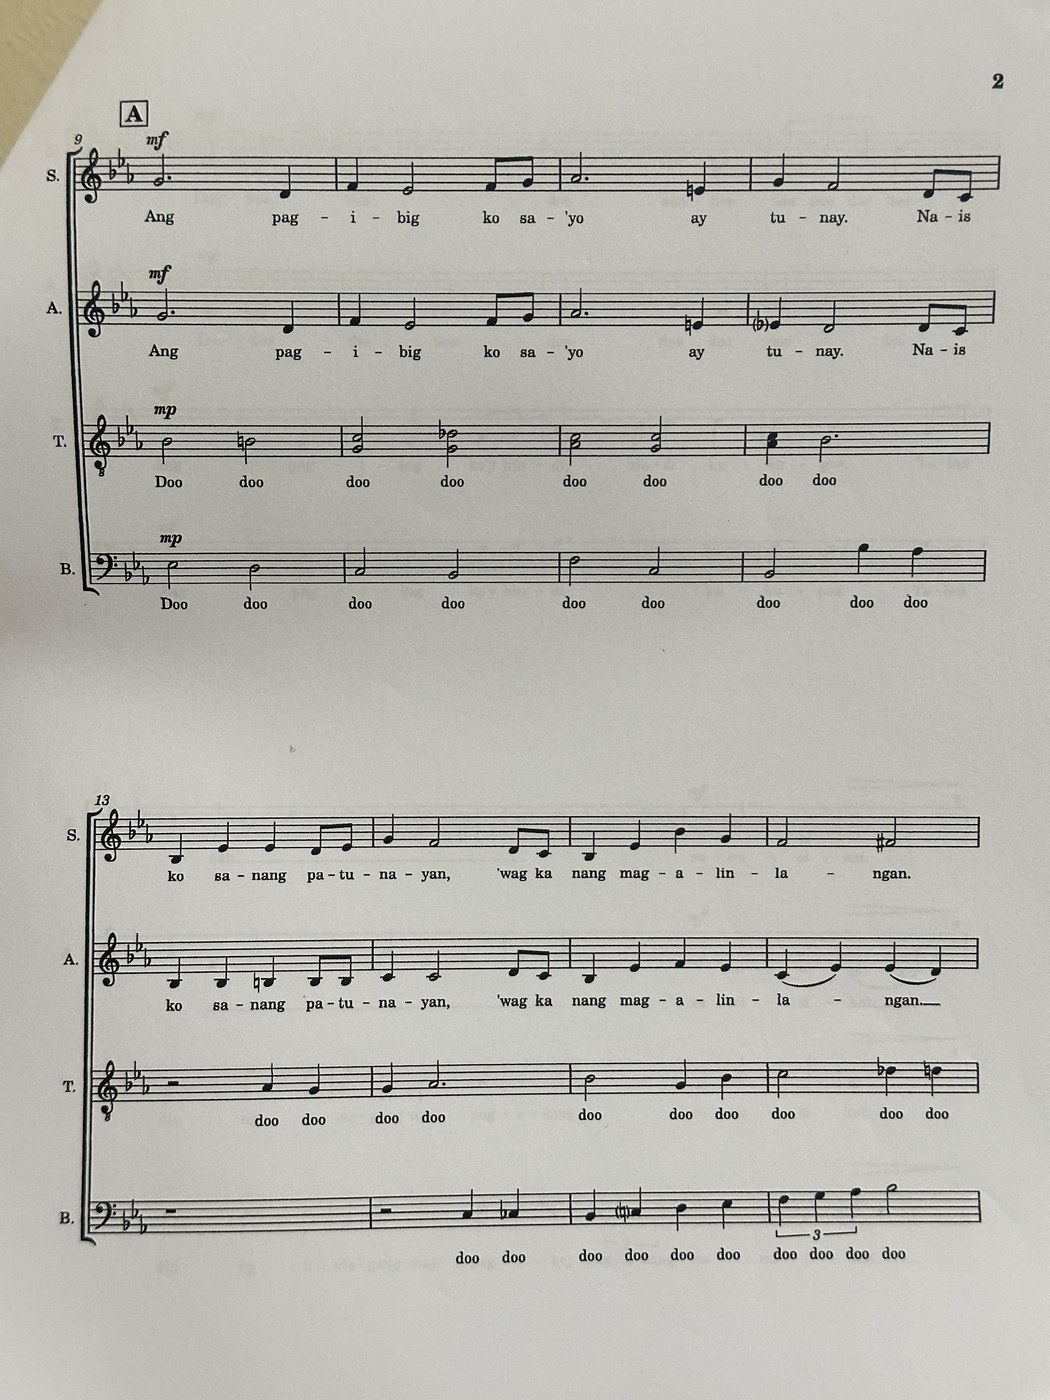
\includegraphics[height=\FigTwoHeight]{fig2b_camera.jpg} \\[-1pt]
{\scriptsize (a)} & {\scriptsize (b)}
\end{tabular}
\end{minipage}

{\figurecaptype
\caption{The same test page (\emph{Gaano Ko Ikaw Kamahal}, p.~2) as
digital render (a) and smartphone capture (b), showing lighting, skew,
and noise artifacts.}
\label{fig:capture}}

\subsection*{3.\enspace Remaining Work}

Remaining work involves (1)~reducing spurious notes and rhythm errors,
which drive the remaining symbol error, and raising camera pitch
accuracy toward the 85\% target; (2)~evaluating on a larger held-out set
of Filipino SATB scores; (3)~completing the Flutter mobile application
and connecting it to the Flask backend; and (4)~a usability evaluation
with Filipino choir members using the System Usability Scale.

\end{document}
